In this section, we describe the data-sets at our disposal, the system parameters we derive from them, and the models by which we evaluate the different policies for the incentive scheme.

\subsection{Data-Sets}

Our analysis relies on three different data-sets. First, we have a list of all trips in the system with origin location, destination location, and respective times of the start and the end of the trip \cite{citibikedata}. Second, we have a list that indicates which of the above trips were rewarded with points by the existing offline incentive policy (as well as whether the point was awarded for the rental, the return, or both) \cite{citibikeInternal}. Last, for each minute and each station in the system, we have the number of bikes reported to be at the station at that time as well as the total number of docks available \cite{citibikejson}.

We use data collected over three different time periods in 2016 in our analysis: 04/01--05/13 (base), 10/03--10/30 (training) and 10/31--12/14 (testing). The base period includes the most recent 6-weeks of data when no incentive program was in use, and represents the system before incentives were introduced. The training period involves the first 20 days of the winter data after incentives were introduced, and the remainder is used as the testing period. The base and training periods are used to help calculate the system parameters, such as the rental/return rates and the stochastic interpretation of the incentives' effect explained later in this section, and also serve as the training period for some of our incentive policy algorithms. The testing period is used to evaluate and compare our suite of policies. 

%Newly added.
%During the time periods from which our data is drawn, two 6-hour time intervals were incentivized in the Citi Bike system: 6AM-12PM and 4PM-10PM - we refer to them as the AM and PM periods respectively. All incentivized trip data comes from these two 6-hour time intervals. The daily total number of incentivized rentals/returns in the AM/PM for the test period are shown in Figure [?], where we see a generally equal distribution of rental/returns in the PM period, but a return-skewed distribution in the AM period. 

%\begin{figure}
%\centering
%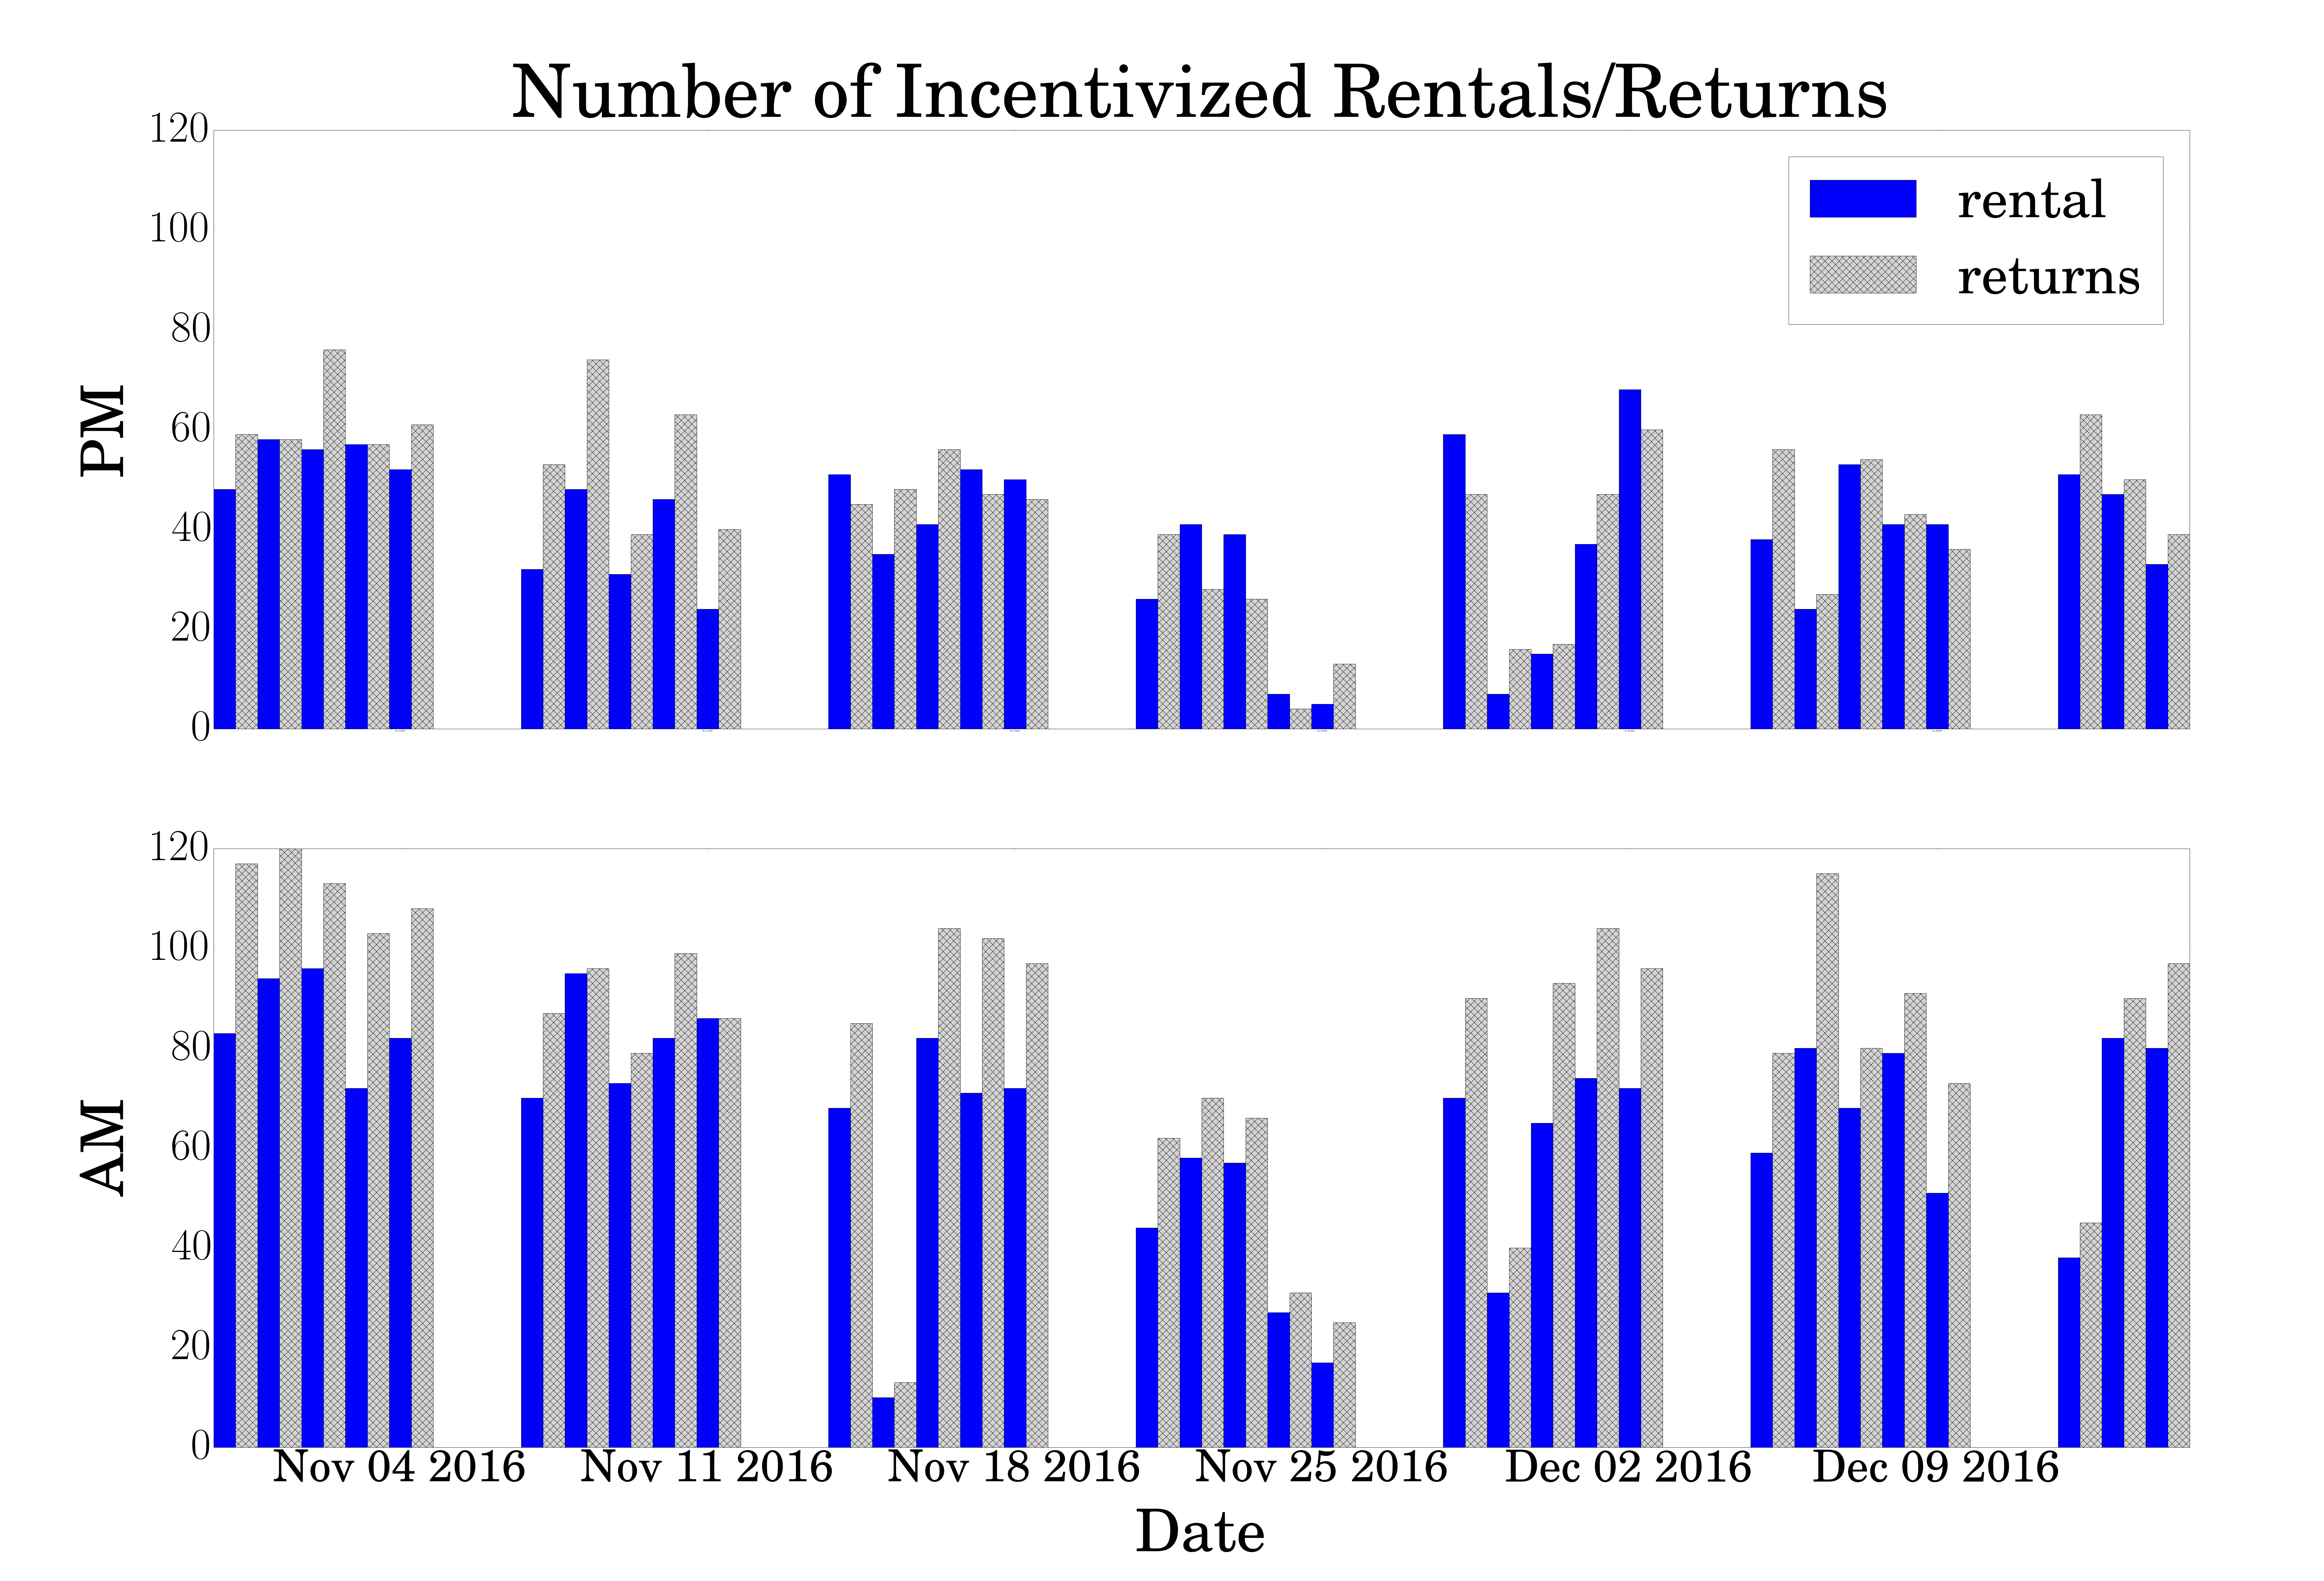
\includegraphics[width=.5\textwidth]{../SubmissionPlots/ActuallyUsed/Rental_Return.png}
%\caption{Total number of incentivized rentals/returns in the test period.}
%\label{fig:Incentivized Rentals/Returns}
%\end{figure}


\subsection{Data Censoring}

In our data, censoring proves to be a challenge as the data does not accurately reflect the true demand within the system. For example, a rider wanting to rent or return a bike to a station, with all docks empty or full respectively, cannot do so; thus, the corresponding demand would not be reflected in our data sets. To account for this problem of demand-censoring, when estimating average rental/return demand, we follow the methodology of \cite{o2015data} and examine station behavior on a minute-by-minute basis, only considering "active rental/return minutes", that is, minutes when a station has non-empty or non-full docks, respectively.

\subsection{Arrival and Departure Rates} 

Our analysis relies on three types of arrival and departure rates: regular-angel, incentive-angel, and non-angel rates. Regular-angel rates are the natural rental/return rates into a station for all angel riders combined, when no incentive is provided. The incentive-angel rates are the rates for the same set of customers when incentives are given. The non-angel rates are the rates for all other customers and are assumed to be unaffected by the incentive program. In our calculation of rates, we follow the work by \cite{o2015data} in assuming that the rates are independent across stations and calculate rates for every half-hour interval of the day starting from 12AM in the units bikes per minute.

To calculate the incentive-angel and non-angel rates, we take the data for a station's previous $q$ weekdays, and divide the total number of all arrival/departure trips by the specified riders by the total "active rental/return minutes" for each half-hour interval. In the results we present, $q$ is set to 20.

Formally, for each day $d$, station $s$, and time index $t$, let ($m_{d, s, t}^-$, $m_{d, s, t}^+$)  denote the active rental/return minutes, ($r_{d,s,t}^{a, +}$,$r_{d,s,t}^{a, -}$), ($r_{d,s,t}^{n, +}$, $r_{d,s,t}^{n, -}$) the number of arrival/departure trips for angel and non-angel riders respectively, and $D(d)$ be the set of the preceding $q$ weekdays before day $d$. Then the incentive-angel arrival rates $\lambda_{d, s, t}^{i, +}$ for day $d$, station $s$ and time index $t$, where $t \in \{0, 1, 2, ..., 47\}$ for the 48 half-hour intervals of the day (e.g. t=12 is 6 a.m.) are calculated as the rate per minute normalized to account for only active minutes, as follows (similar for departure rates $\lambda_{d, s, t}^{i, -}$ and non-angel arrival/departure rates $\lambda_{d, s, t}^{n, +}$ and $\lambda_{d, s, t}^{n, -}$):
\begin{equation}
\lambda_{d, s, t}^{i, +} =   \frac{\sum_{d' \in D(d)} r_{d',s,t}^{a, +}}{\sum_{d' \in D(d)} m_{d',s,t}^+} 
\end{equation}

%we define ($\lambda_{d, s, t}^{i, +}$, $\lambda_{d, s, t}^{i, -}$), ($\lambda_{d, s, t}^{n, +}$, $\lambda_{d, s, t}^{n, -}$) and ($\lambda_{d, s, t}^{r, +}$, $\lambda_{d, s, t}^{r, -}$) to be the pairs of incentive-angel, non-angel and regular-angel rental/return rates respectively for day $d$, station $s$ and time index $t$, where $t \in \{0, 1, 2, ..., 47\}$ for the 48 half-hour intervals of the day (e.g. t=12 is 6 a.m.). Further,


To estimate the regular-angel rates we used data from the base period, when no incentive program was offered. The regular-angel rates are assumed to be identical across days, and are calculated by dividing the angel rider's total number of all arrival/departure trips by the total "active minutes" in the base period for each half-hour interval, and applying a correction factor. The correction factor, $U$,  accounts for any general macro-change in system usage from the base time period to our testing time period. The correction factor is calculated by dividing the average daily total number of trips by non-angel riders during the training period by their average daily total number of trips during the  base time period. Finally, because the correction factor is an estimate of the change, we capped the regular-angel rates to be at most the incentive-angel rates to reflect our prior beliefs that incentivization actually helps our system. If we define $D$ to be the set of weekdays in the base time period and $U$ to be the correction factor, the regular-angel arrival rates are calculated as follows (similarly for departure rates):
\begin{equation}
\lambda_{d, s, t}^{r, +} = min(U \cdot  \frac{ \sum_{d' \in D} r_{d',s,t}^{a, +}}{ \sum_{d' \in D} m_{d',s,t}^+} , \lambda_{d,s,t}^{i, +} ) 
\end{equation}

\subsection{Stochastic View of Incentives}
Our analysis also relies on the probability that an incentivized rental/return would not have occurred if it had not been for the incentive; in particular, the rebalancing due to a rental/return that happens regardless of the incentives should not be attributed to the incentive scheme. We compute these probabilities for each day, station and half-hour interval by % and represents the probability that an incentive trip in this time-interval occurred due to the incentive. 
%To calculate them, 
dividing the difference of the incentive-angel and regular-angel rates by the incentive-angel rate. Formally, with $p_{d, s, t}^+$ and $p_{d, s, t}^-$ denoting the probabilities that a rental/return was triggered by the incentives, we compute these probabilities as %  and departure trip respectively, the probabilities of a rental/return occurring due to the incentives are calculated as follows (similarly for departure):
\begin{equation}
 p^+_{d, s, t} =  \frac{\lambda_{d, s, t}^{i, +} - \lambda_{d, s, t}^{r, +} }{\lambda_{d, s, t}^{i, +}}
 \end{equation}

\subsection{User Dissatisfaction Function}\label{ssec:udf}
The user dissatisfaction functions defined by \cite{raviv2013optimal} map the number of bikes at a station at a given time to the expected number of out-of-stock events over the course of a subsequent finite time-horizon. Formally, the functions assume that two exogeneous stochastic processes create arrivals of customers intending to return and rent bikes at the station. In our implementation, the stochastic processes are given by time-varying Poisson processes with rates being the non-angel rates. Crucially, the processes are assumed to be independent of the initial condition, that is, of the number of bikes at the station at the beginning of the time horizon. Then, each intended rental decreases the number of bikes in the station by 1 if a bike is available, i.e., if the number of bikes is at least 1. Intended returns increase the number of bikes by 1 if an empty dock is available at the station, i.e., if the number of bikes is less than the capacity of the station.  

Customers experience out-of-stock events if they intend a rental and the station is empty or if they intend a return and the station is full. Given the non-angel rental and return rates, one can then compute for a given station $s$ with $\ell$ bikes at time-index $t$, the expected number of out-of-stock events over a time-horizon beginning at time-index $t$, i.e., the expected number of intended returns  when the station is at capacity plus the expected number of intended rentals when the station is empty. We denote this expectation by $\phi_{s, t} (\ell)$.

%EXPLAIN HOW THE UDF USES DATA TO BE COMPUTED (NO DETAILS).

%In order to 

\begin{figure}
\centering
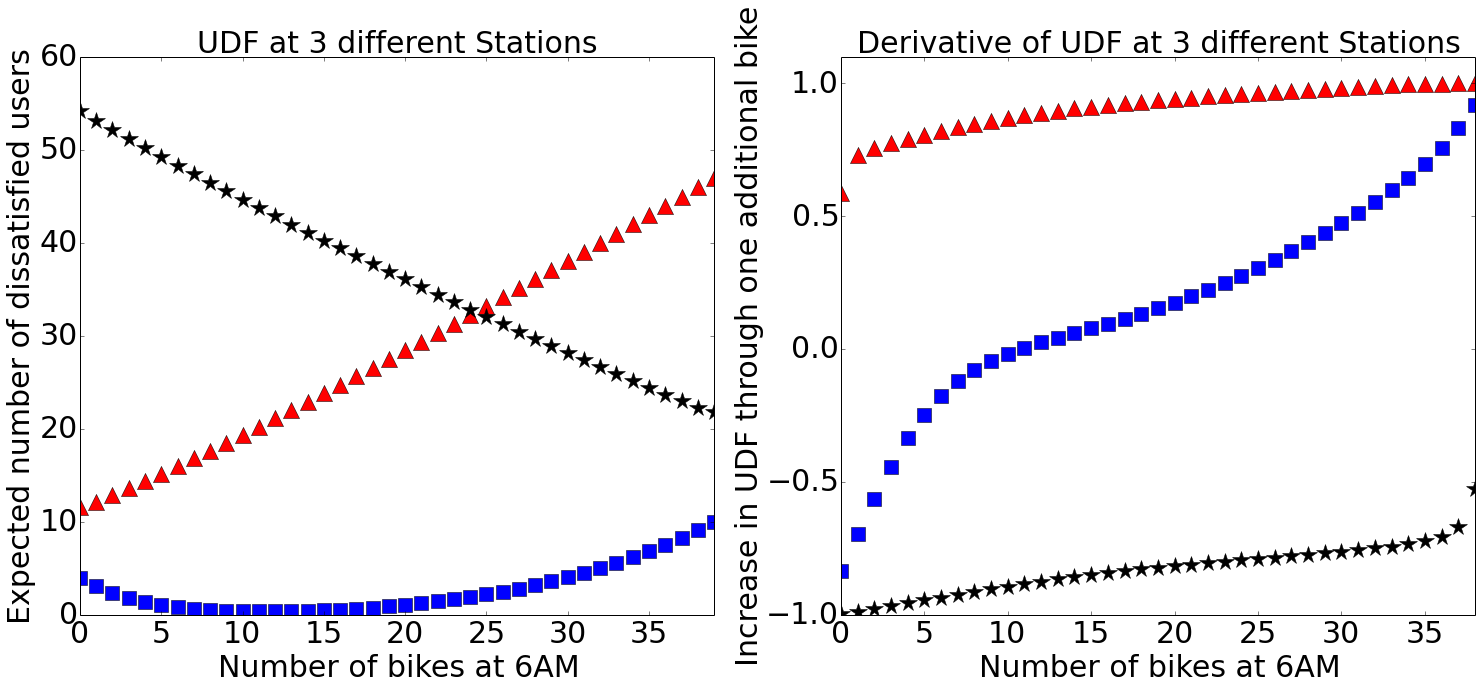
\includegraphics[width=.5\textwidth]{../Plots/UDFandDerivative2.png}
\caption{User dissatisfaction function $\phi_{s,t}(\cdot)$ and its discrete derivative for 3 different stations $s$ with the same capacity.}
\label{fig:UDFandDerivative}
\end{figure}

%Formally define the model as defined by \cite{raviv2013optimal}, describe the partition into half-hour intervals, emphasize that there's no point in taking smaller intervals, describe

\subsection{Performance Metrics and Policies}

For each incentivized return, we can estimate the reduction in out-of-stock events by computing the discrete derivative of the user dissatisfaction function with respect to one additional bike, evaluated  as a function of the number of bikes present in the station before the arrival. Similarly, for incentivized rentals, the estimated reduction in out-of-stock events equals the difference in the value of the user dissatisfaction function evaluated with one bike less and the actual number of bikes in the station.  In Figure \ref{fig:UDFandDerivative}, we display the respective user dissatisfaction functions and the value of the derivatives for three different stations at 6AM. Evaluating the user dissatisfaction functions for every half-hour interval, we estimate the impact of each rental/return on future out-of-stock events by evaluating the derivative of the user dissatisfaction function for that time-interval at the number of bikes present at the time of the return (and similarly for rentals). If we let $\delta_r$ denote the estimated reduction on future out-of-stock events for trip $r$,  let $\ell$ denote the bike-level at the station before the trip completed, and let $s$ and $t$ denote the station and time-index associated with the trip, we find that we may compute $\delta_r$ for a return as follows (similarly for rentals):

\begin{equation}
\delta_r = \phi_{s, t} (\ell) - \phi_{s, t} (\ell + 1)
\end{equation}

%The overall performance metric for a policy is defined to be the expected total reduction in out-of-stock events less the costs for any incentives given.  With the user dissatisfaction functions, we can estimate the impact of a single incentivized trip. More specifically, f

Though $\delta_r$ captures the impact of a return (rental) on the estimated number of out-of-stock events, it lacks two important aspects for our analysis. First, it lacks the cost associated with the incentive itself. To capture the operator's cost of the incentive scheme in the form of electronic gift cards, membership extensions, and other rewards (cf. \cite{bikeangels}), we include a constant cost parameter $\beta$ for every point awarded by an incentive scheme. Second, for every incentivized rental (return), we can incorporate the probability $p_{d,s,t}$ that the rental (return) would not have occurred without an incentive given; here, $d, s, t$ is the date, station and time index respectively in which the rental (return) occurred. This gives a stochastic perspective of the causal effects of incentives, in contrast to the deterministic assumption that incentivized rentals (returns) are always caused by the incentive. Using the above, we can define for every single incentivized return (rental) the performance of incentivizing it with both the deterministic and the stochastic perspective as % we can define the performance of incentivizing it by either viewing 

%In order to include the %As we consider the expected impact of a trip, it is worthwhile to not only include the impact of each incentivized trip on the user dissatisfaction functions, but also the 
%likelihoods that trips would have occurred without the incentives, we use the NEED A NAME FOR THESE IN STOCHASTIC VIEW OF INCENTIVES to define a stochastic and deterministic performance metric for a single trip. The deterministic evaluation assumes all incentivized trips occur due to  the incentive scheme only, and the expected reduction in out-of-stock events equals $\delta_{r}$ itself. The stochastic evaluation takes into account the probability of the trip occurring due to the incentive, and calculates the expected reduction to be $\delta_{r} * p_{d,s,t}$, where $d, s, t$ is the date, station and time index respectively in which the trip occurred. 

%Furthermore, when evaluating the performance metric for a policy we not only want to consider the expected impacts of the incentivized trips, but also account for the cost of giving incentives. Thus, we associate a fixed cost $\beta$ per awarded incentive point. This corresponds to the operator's cost of monthly rewards in the form of electronic gift cards, membership extensions, etc. \cite{bikeangels}.

%Let us define $\Delta_{r}$ to be the expected reduction on future out-of-stock events minus the cost of incentivizing for trip $r$. The deterministic and stochastic evaluation of $\Delta_r$ is calculated as follows:
\begin{equation}
    \Delta_r=
    \begin{cases}
       \delta_{r} - \beta & \text{ if deterministic}\\
       \delta_{r} \cdot p_{d,s,t}  - \beta & \text{ if stochastic}
    \end{cases}
\end{equation} 

Given $\Delta_r$ as a performance measure for incentivizing a single return (rental) $r$, we define the performance of a policy as the sum of all $\Delta_r$ corresponding to incentivized rentals (returns) $r$. Formally, denoting by $\tau$ the set of all rentals (returns) in the testing period, we define a policy $P$ as a function $P:\tau\to \{0,1\}$ identifying for each rental (return) $r$ whether or not $P$ incentivizes it. Then,   %   let us define a policy to be a mapping from the set of incentivized trips to the binary decision variable indicating whether a trip is incentivized. Thus let us define $\tau$ to be set of possible incentive trips, and a policy $P$ to be the function $P: \tau \to 0/1$.
to compute the overall performance $H(P)$ of a policy $P$ we compute
\begin{equation}
 H (P) =  \sum_{r \in \tau} P(r) \cdot \Delta_r 
\end{equation}



%Explain the set up of the problem, data collection methods \\
%Explain the Cost Curve function and what it represents \\
% \\
